\documentclass{article}
\usepackage[utf8]{inputenc}
\usepackage[italian]{varioref,babel}
\usepackage[colorlinks]{hyperref}

\hypersetup{linkcolor=red, urlcolor=green, pdfauthor=Nazif Bajramoski} 

\usepackage{lipsum}

\usepackage{fancyhdr}
\pagestyle{fancy}

\usepackage{marginnote}
\usepackage{graphicx}
\usepackage{tabularx}


\lhead{}
\chead{}
\rhead{}

\lfoot{}
\cfoot{}
\rfoot{\thepage}
% Piè di pagina.

\renewcommand{\headrulewidth}{0 pt}
\renewcommand{\footrulewidth}{0.3pt}
% Comandi che permettono di inserire la riga che separa l'intestazione e il piè di pagina dal testo con una riga (spessa 0.3 punti).

\title{Progetto interdisciplinare}
\author{Nazif Bajramoski, Benjamin Travaglin, Christiam Gharib, Jonas Adam}
\date{\today}
% Indicazioni per il titolo, l'autore e la data.

\begin{document}

\maketitle

\newpage

\tableofcontents

\newpage

\section{Introduzione generale al progetto}
Come ogni anno, alla scuola cantonale di commercio, gli allievi devono svolgere un lavoro di maturità a gruppi, chiamato anche comunemente progetto interdisciplinare. Questo lavoro viene svolto attraverso un processo di ricerca che comprende la raccolta di materiale, analisi di dati statistici, interviste, sondaggi, ricerche approfondite in rete, lettura di testi e documenti che possano rispondere ad una domanda di ricerca precisa, che è stata fissata all’inizio del corso.
L’argomento principale, sul quale è stato svolto il nostro lavoro, è “l’Economia a km 0”. Per introdurre il corso abbiamo visionato un film documentario dal titolo “Domani”, il quale ci ha permesso di identificare diverse possibili tematiche come la riqualificazione urbana, gli orti urbani, la moneta locale e gli scambi dal produttore al consumatore, tra quest’ultime abbiamo focalizzato la nostra attenzione sulla riqualificazione urbana del nuovo agglomerato di Bellinzona.
Ci siamo interrogati su quali possono essere le esigenze della popolazione e quali sono le migliorie che possono essere apportate al nuovo agglomerato per il bene comune; dunque abbiamo voluto approfondire le nostre conoscenze sull’urbanistica e su come riqualificare il territorio. 


\section{La riqualificazione urbana}
\subsection{Definizione}
Prima di addentrarsi nel vivo dell’argomento è necessario dare una definizione precisa di che cosa sia la riqualificazione urbana e in seguito che cosa significhi per noi.
Con riqualificazione urbana si intende, in primo luogo, dare una nuova immagine allo spazio edilizio già esistente in una determinata zona geografica. Si possono racchiudere in essa diversi interventi che fanno parte di una rigenerazione, ad esempio nelle zone più degradate, interventi che possano limitare il consumo di territorio ma allo stesso tempo che rispettino l’ambiente e il paesaggio circostante, soprattutto nell’ambito della sostenibilità. Le funzioni urbanistiche sono molto importanti e comprendono diversi aspetti come l’organizzazione delle parti urbane e il collegamento con le zone periferiche, la creazione di nuove centralità di svago, la revisione delle infrastrutture stradali e pedonali.
Spesso la condizione delle moderne periferie non è delle migliori, diversi sono i motivi che portano ad avere una situazione simile, basti pensare alla disomogenea organizzazione morfologica, il collegamento assente fra periferia e città, ma soprattutto una gestione poco efficacie degli spazi. 

\subsubsection{L'urbanistica}

\subsubsection{Mobilità e sicurezza}

\subsection{Cosa significa per noi}
\subsubsection{Definizione di benessere}

\subsection{Casi ed esempi reali}
\subsubsection{riqualifica della foce di Cassarate}
\subsubsection{riqualifica delle Lorelei }
\section{Commenti dati USTAT}
Per inquadrare il nuovo comune nato dalla fusione di realtà diverse, abbiamo ritenuto opportuno proporre un’analisi quantitativa della popolazione e dell’occupazione 
Questo approccio  è necessario se si vuol parlare di riqualifica urbana in quanto permette di conoscere con accuratezzale dinamiche e la particolarità dei diversi quartieri, all’interno della nuova realtà comunale. Capire deve sono i luoghi di lavoro e dove invece quelli residenziali, permette poi di pianificare la nuova città, creando le interconnessione necessarie per migliorare la qualità di vita delle persone

\subsection{Analisi demografica}
Attraverso un’analisi dell’evoluzione della popolazione dal 1990 fino al censimento più recente del 2016 si è arrivati a diverse conclusioni. L’incremento maggiore è stato registrato  nei comuni di Claro, Monte Carasso, Gnosca e Gudo; raggiungendo una variazione attorno al 70\%.  Mentre al centro (Bellinzona e Giubiasco) la crescita è stata poco rilevante. In questi 27 anni, la popolazione ha emigrato verso le zone periferiche della città dove i costi degli immobili sono inferiori ma, forse, alla ricerca di calma e tranquillità. Queste dinamiche comportano però spostamenti quotidiani dal luogo di residenza a quello lavorativo nel coso i due luoghi non coincidono come nel nostro caso (confronto tra tab. 1 e 2) . L’utilizzo della vettura privata per spostarsi concentra il traffico nelle ore di inizio e fine lavoro. La creazione di una via intelligente e alternativa destinata alla mobilità lenta è necessaria (assieme naturalmente all’ampliamento dei servizi pubblici). Con la realizzazione di una vera propria rete di piste ciclabili che collegano la periferia al centro di Bellinzona.

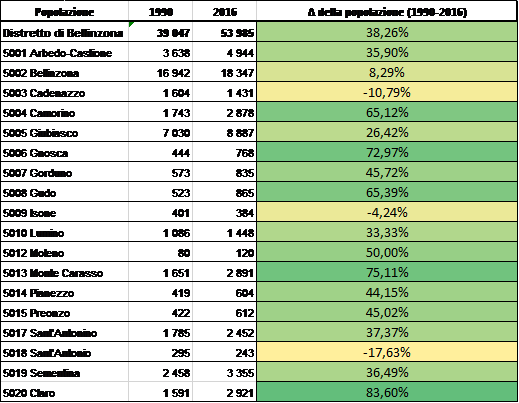
\includegraphics[scale=0.5]{Capitoli/immagine progetto.png}

\subsection{Analisi economica}
Per analizzare il nuovo comune sotto l’aspetto economico, si possono prendere i dati dell’ufficio cantonale di statistica che riguardano i lavoratori a tempo pieno. Si può notare una variazione importante nei comuni di Arbedo – Castione (62,5\%) (che non fa però parte del nuovo comune) e nei due piccoli comuni di Moleno e Sant’Antonio (ma i valori in termini assoluti sono irrilevanti). Mentre dove l’impiego è aumentato in maniera considerevole sono i comuni di Monte Carasso (588 posti di lavoro a tempo pieno, +34,4\%), Cadenazzo (1404, +18.9\%), Sementina (795, +17,6\%), Tuttavia la maggior poste dei posti di lavoro sono concentrati a Bellinzona (53\%) e, in minor misura, Giubiasco (12\%). Inoltre, solo una piccola minoranza ha la possibilità di lavorare nel luogo dove risiede e questo comporta continui spostamenti giornalieri.  
\\
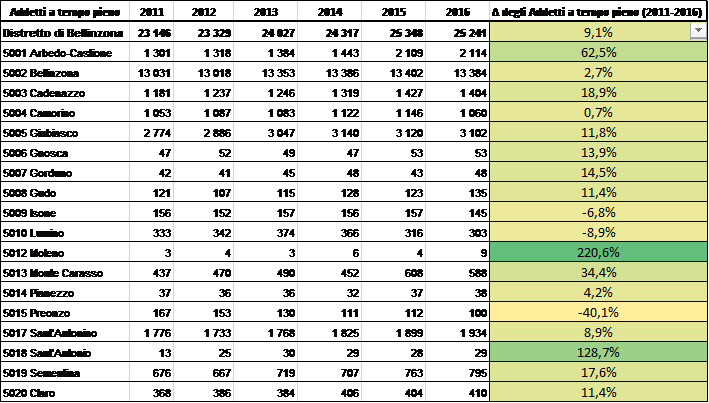
\includegraphics[scale=0.5]{Capitoli/ioioi.png}
\\Un confronto possibile è il rapporto abitante – posto di lavoro del distretto di Bellinzona in confronto con la percentuale Cantonale e quella Nazionale.

----TABELLA---
\\
La città di Bellinzona si trova al di sopra della media Svizzera, grazie ai numerosi uffici amministrativi cantonali, mentre il distretto di Bellinzona ha un rapporto inferiore in quanto all’interno del distretto vi sono dei quartieri nella quale sono perlopiù residenziali e quindi non offrono un impiego. Attenzione: città o quartiere, distretto o città?

\subsection{Conclusione}
Questa breve analisi evidenzia un problema comune a tutte le città: nei centri ci sono la maggior parte dei posti di lavoro mentre la popolazione tende a spostarsi nelle periferie dove i costi dell’alloggio sono inferiori. La contropartita a questa evoluzione è naturalmente un incremento del traffico. Nel caso specifico di Bellinzona il problema è poi amplificato dal traffico proveniente da fuori, legato ai numerosi posti di lavoro nella Pubblica amministrazione. Limitandoci alla popolazione urbana, è però possibile contenere il problema incrementando la mobilità lenta con piste ciclabili efficaci.
Anche perché su percorsi brevi (attorno ai 5-8 km) la biciletta ha tempi di percorrenza inferiori a quella dell’auto negli orari di punta, naturalmente a condizione che esistano delle piste ciclabili adeguate. Naturalmente anche i mezzi pubblici possono essere efficaci, ma richiedono più investimenti e interventi importanti per renderli competitivi.
Nel seguito del nostro lavoro, ci concentreremo soprattutto sulle piste ciclabili, perché possono ridurre il traffico veicolare ma soprattutto perché potrebbero essere un ottimo strumento di connessione e legame tra i vari quartieri.

---TABELLAA---


\section{Progetto di riqualificazione urbana per il Bellinzonese}

\subsection{Introduzione}

\subsection{Ciclopiste}
Durante la pianificazione delle ciclopiste si deve considerare, oltre che della loro funzione di interconnessione, diversi elementi che le rendono a norma, sicure e agibili. Infatti, bisogna tenere conto delle diverse norme che ne regolamentano la creazione. I percorsi ciclabili rappresentano, per i ciclisti, un grosso vantaggio, in quanto separano il traffico lento, da quello a motore, aumentando il confort, la sicurezza e riducendo lo stress. Elementi che si muovono a favore di questo sviluppo sicuro possono essere la segnaletica stradale, pannelli informativi, stampati e internet. Le piste ciclabili possono avere più funzioni, la prima è la mobilità quotidiana (spostamenti funzionali), la seconda è la funzione turistico-ricreativa. Queste due categorie devono essere sviluppate in modo differente, quelle relative allo spostamento quotidiano devono avere un carattere funzionale, efficiente e devono raggiungere i principali centri di lavoro/scolastici; quelli con uno scopo turistico-ricreativo invece non devono rispettare particolari percorsi o destinazioni, in quanto la strada è essa stessa la meta da raggiungere, questi percorsi devono quindi offrire un’esperienza attrattiva con paesaggi e punti di sosta tranquilli. 
La segnaletica, all’interno di un percorso ciclabile, deve permettere di seguire la direzione desiderata senza difficoltà, riducendo al massimo le interruzioni, oltre a ciò ha la funzione di rendere il percorso attrattivo. Grazie ad una buona segnaletica, infatti, le piste diventano più sicure, attrattive e veloci, inoltre diventano più facilmente reperibili, anche da turisti o persone che non sono residenti del posto. 
\\
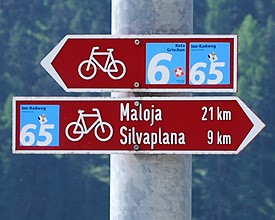
\includegraphics[scale=1]{Capitoli/cartelol.jpg}
\\
Essendo la bici un mezzo di trasporto non dotato di motore, le soste, le deviazioni e in generale gli spostamenti non scorrevoli, implicano una perdita di tempo e soprattutto di energie. Per rendere lo scorrimento di queste piste il più ottimale possibile, l’obiettivo è di minimizzare al massimo il numero di soste durante la percorrenza di una via ciclabile. Problemi che possono influenzare negativamente la qualità del percorso possono essere le geometrie sfavorevoli, topografia sfavorevole, soste di breve/lunga durata (semafori/passaggi a livello). 
Per la creazione della pista ciclabile ottimale, è quindi necessario tenere in considerazione una moltitudine di elementi. 
In Svizzera le piste ciclabili sono rappresentate in colore rosso. Per i percorsi creati nel progetto di riqualifica urbana del territorio bellinzonese, è necessario che la segnaletica sia puntuale e precisa, infatti tutti i nuovi percorsi dovranno essere marcati dettagliatamente e adeguate secondo la regolamentazione consigliata. 
Sempre in più parti del mondo il sistema del traffico viene modificato al fine di permettere l’agevolazione dei mezzi di trasporto lento, un esempio molto prossimo alla nostra realtà, è la nuova struttura della rete stradale di Lugano, che ha permesso ai mezzi di trasporto pubblici e ai ciclisti di coesistere con una maggiore armonia rispetto al precedente modello di rete urbana.  Tuttavia ha scaturito effetti collaterali nei confronti delle abitudini dei conducenti, per questa ragione andrebbero considerate anche queste conseguenze, per prevenire eventuali problemi anche nel territorio in cui si vorrebbe effettuare queste modifiche

\subsection{Traffico bellinzonese, evoluzione dal 1991 al 2017}
Grazie ai dati forniti dall’osservatorio ambientale della Svizzera italiana si può constatare come gli ultimi 20/30 anni abbiamo assistito un importante incremento del traffico. I dati che coprono, generalmente, un periodo che va dal 1991 al 2017, evidenziano la situazione dei nuovi quartieri del comune di Bellinzona. Come si vede dal grafico 1 (la numerazione di grafici e tabelle dovrà essere progressiva e secondo il capitolo, ad esempio 4.1) l’aumento è stato significativo per tutti i punti di rilevamento.  Le cause di questo aumento possono essere varie: aumento della popolazione nelle zone urbane, aumento dei posti di lavori nel quartiere di Bellinzona, incremento del traffico automobilistico e lo sviluppo economico. 
Dare una risposta unica e definitiva è evidentemente difficile ma è chiaro che la pressione del traffico sul centro del nuovo comune è aumentato – oltretutto su una rete stradale che è rimasta praticamente uguale negli ultimi decenni – nonostante le politiche per favorire il trasporto pubblico.

\input{Capitoli/Capitolo5.tex}

\end{document}